% binding info: NO NOTEBOOKS OR RING BINDERS, proefssional appearance, non-paper cover, bound. 8.5x11 w/ 1 inch margins, left side 1.5in margin.

% This is a test comment. So stop reading it you piece of shit

% text formatting info: The paragraphs are to be fully justified (both left and right sides). New paragraphs may begin by indenting the line or by not indenting but leaving a space. However, DO NOT do both. The body font must be Times Roman, Arial, Helvetica, or be approved by the instructor with a font size of 10-12 pts. Heading fonts can be no larger than 20 pts. The document must be single-spaced and printing can be single or double sided. Color printing is optional and left to the discretion of the groups.

% sources info: 5. The appendix must contain written authorization (emails, letters, or explicit permission citations) for rights to include or use copyrighted content. 6. All copyrighted contents must display the content’s origin or author, and an appropriate phrase such as “reprinted with permission.” 

% citing info: 7. All elements of the document that support the written text, such as figures, table, illustrations, code segment, charts, etc., must be cited in the body of the text, and the citation must appear before the element is shown. Supportive elements cannot begin a chapter, section, or paragraph. All supportive material must be captioned, which include the element name and number and a description. If you do not author the element, the caption must contain wording identifying that you have permission to use the element. The actually permission authorization must be included in the appendices.

% reference format info: 8. Your document should contain a “References” section at the end that lists all of the source material cited in your document. The references should be listed in the order that they first appear in your document in a format like the following (first is a book, second is an article): [1] J. Hennessy and D. Patterson. Computer Architecture: A Quantitative Approach, 5 th edition, Morgan Kaufman publishers, 2014. [2] M. Heinrich et al. “The Performance Impact of Flexibility in the Stanford FLASH Mujltiprocessor”, In Proceedings of the 6th International Conference on Architectural Support for Programming Languages and Operating Systems (ASPLOS), pages 274-285, 1994

% citation formatting: When citing the references in the text use a non-breakable space (e.g. Ctrl-shift-space in Word, \&; in HTML) before the citation and then square brackets and the number: Some researchers say that the occupancy of the node controller is the parameter most critical to the performance of the overall machine [2]. If you want to cite multiple references at once just separate them by commas like so [1,3,7].

\documentclass[a4paper,10pt]{article}
\usepackage[utf8x]{inputenc} 
\usepackage{graphicx}
\usepackage{float}
\usepackage{geometry}
	\geometry{
	letterpaper,
	total={8.5in,11in},
	left=1.5in,
	top=1in,
	right=1in,
	bottom=1in
}

%opening
\pagenumbering{roman}
%1. Cover page with title, group number, team members, date, and any other relevant information, such as participating organizations and sponsors.
\title{Group 12 Project Final Design Document}
\author{Eric Momper, Peter Lomason, John Barber}
\setlength{\parindent}{0pt}
\begin{document}
	
	\maketitle
	
	\pagebreak
	\tableofcontents
	\pagebreak
	
	\section{Introduction}
		Our Project is intended to be a psychological theraputic tool that helps patients through simulation in Virtual Reality.
	Many of the new up and coming Virtual Reality devices look very promising at providing better and more realistic immersion and simulation for users at a lower cost than ever before. We aim to bring psychological tools to the home of the average user. This will allow those seeking certain therapies or treatments to perform them more often since such services often require high diligence and repetition to produce results.
	
	\paragraph{A few of these devices include:}
	\begin{itemize}
		\item Oculus Rift, Oculus Touch
		\item HTC Vive
		\item Samsung Gear VR
		\item Google Cardboard
		\item Microsoft Hololens
	\end{itemize}
	
	\paragraph{ Some of our project ideas are related to the following:}
	\begin{itemize}
		\item ​Immersion Therapy for phobias, dysphorias, or PTSD (Virtual or Augmented Reality)
		\item Therapy for burn victims, phantom pain for amputees,  (Virtual Reality)
		\item Creating a calm environment for  anxiety disorders, or autism (Virtual Reality)
		\item Creating a drawing art therapy tool that allows for creativity in 3D space (Virtual or Augmented Reality)
	\end{itemize}
	
	
	\paragraph{Project Direction} ~\\ We are currently contacting faculty in the psychology department for collaboration or guidance on opportunities to use our project for helping their patients or for their research.
	\paragraph{Integration} ~\\ Our project will be created in Unity, Unnreal Engine, or written with a C++ OpenGL/ DirectX SDK wrapper, depending on the direction of our design, and the VR device we have available. It will most likely be windows exclusive as many VR devices are dropping Linux and OSX support unless we can find some options that will provide cross platform systems, which is said to be available in the near future for some platforms but not currently finished.  
	
	\pagebreak
	
	\section{Status of Virtual Reality in Psychology}
	The first use of Virtual Reality therapy in Psychology was in 1995 by psychologist Barbara Rothbaum and computer scientist Larry Hodges. T
	hey found that virtual reality therapy could help patients overcome phobias such as arachnophobia or a fear of heights. Since then many others 
	have used virtual reality as a tool in psychology. The main use of virtual reality in psychology is a form of treatment called Exposure Therapy. 
	This type of treatment can be used to address psychological issues such as Autism spectrum disorder, Obsessive Compulsive Disorder, various phobias, 
	post-traumatic stress disorder, and phantom limb pain. The greatest issue facing treatment with Exposure Therapy is that it requires a high level of diligence and
	repetition. Typically patients cannot make time for appointments as frequently as is required.
	
	\subsection{Immersion Therapy}
	This psychological treatment helps patients simulate past or hypothetical events so they can adapt to or reason through
	various situations. Our paticular area of foucs is fear of heights (Acrophobia).
	\subsection{Pain Treatment}
	Some examples of this are used with burn victims or people with acute pain, putting them in a calming or cold environment to distract them to relieve pain.
	\subsection{Creating a Calming Environment}
	This can be useful for many patients with anxiety disorders as it will allow users to be in a relaxing environment with softer stimuli that can take their mind off of anxiety issues. 
	\pagebreak
	
	
	\section{Team Member Motivations}
	\subsection{Eric Momper}
	My personal motivation for this project is that it is similar to some of the programming I do on my internship (OpenGL and OpenCL image GPGPU processing).
	I also have taken computer graphics with Professor Leinicker and I am currently taking robot vision with Doctor Lobo. This project will be very interesting to me as  
	I will be working with new technologies and programming on a new type of 3D graphics platform. I am also looking forward to studying the psychological benefits
	of Virtual Reality on patients with various disorders.  
	
	\subsection{John Barber}
	This project was my idea, and combines two different fields, virtual reality and psychology.  In the same way, i'm interested in both 
	sides separately, and really hopeful about how they can be combined.  Virtual Reality is exciting to me as a game designer, 
	and one of my closest friends went to work for Emblematic Group, and we've been comparing notes on the future of virtual reality since.  
	However, I also have seen a number of my friends struggle with psychological issues, and have been hoping to find a way to use my Computer 
	Science degree after I graduate to help people.  This is an opportunity to not only accomplish that now, pushing the field forward and finding 
	new ways to use it for people, but also to train myself and find opportunities and connections for the future.
	\subsection{Peter Lomason}
	My interest in this project mainly comes from past experience with virtual reality tools. I used to own an Oculus Rift DK1 and at the time I had it, 
	I was not knowledgeable enough to develop for it. Now I would like to apply what I have learned at UCF to virtual reality development. I eventually want to be
	a video game developer and virtual reality for psychology shares many aspects with that. Being able to program an environment, objects, and interactions is very
	interesting to me and this project will allow me to strengthen my ability to do these tasks.
\pagebreak



\pagenumbering{arabic}

%Project Documentation Guidelines
%additions / deletions where appropriate

%2. Executive summary: An administrative and technical abstract, which includes a brief description of the project, the project objectives, and the technical approach. This is really an overview of 3A, 3B, 3C, and 3D. This is page number 1.
\section{Executive Summary}

\pagebreak
%3. Technical content (This is NOT an outline, just a list of what needs to be included)
%A. Identification of the project and its significance, motivation, etc. (mostly text). Please include personal motivation statements for each project member here. Also you MUST include a separately labeled section or subsection with the title “Broader Impacts” that describes in a minimum of 1 paragraph, the broader implications or impact of your project on society both local and global. How might your project impact underrepresented groups (within science and technology (STEM) or society as a whole), the disabled, non-profit organizations, the environment, diversity, increased participation in STEM fields or the workforce, public engagement in STEM areas, improved national security, enhanced infrastructure, or improved education are all examples.
%B. Technical objectives, goals, specifications, and requirements (mostly text and numbers) FIRST PAPER HERE EZPZ
\section{Project Goals and Objectives}
	Design an environment in Virtual Reality that can be customized and used to help a variety of psychological conditions, and further psychology research, that is accessible to the typical user so they may conduct their own treatment on their own time.
	\begin{itemize}
		\item Increase our understanding of psychology principals \& problems and how virtual reality can help certain conditions.
		\item Find a platform that we can develop on, that creates a high quality virtual reality experience, and is reasonably up to date with modern graphics. Currently our best candidate is the Unity Engine.
		\item Integrate some level of user intractability in the created virtual environments. 
		\item Procedural generation of environments with parameters that can be customized by the user. 
		\item Include pre-constructed environments similar to current treatment strategies in the VR Psychology industry.
	\end{itemize}
	\section{Broader Impacts}
	%Broad implications and impact on society (impact on underrepresented? within STEM and or society as a whole? disabled? non-profit orgs? environment? diversity? increased participation in STEM or workforce? public engagement in STEM? improve national security? enhanced infrastructure? improved education?)
	
	%qualitative, avoid numbers, conceptual discussion specific to project. example descriptions "“lightweight, portable, programmable, low cost, flexible, high resolution, scalable, low power, accurate, mobile, peer-to-peer, autonomic”
	
	Our project would have an impact on the field of psychology as it relates to certain emotional disorders or struggles and the deployment of self-administered therapy for those disorders. It would not only be relevant to people diagnosed with a psychological condition, but also those seeking stress relief or a unique environment to immerse themselves in. By bringing treatment therapies to the end user in their own home and allowing them to perform therapy at their leisure we will have an impact on many people seeking these services who may not have the time to schedule appointments or those who simply won't try due to the stigma surrounding therapy.
	
	
	
	\pagebreak
%D. Detailed design reqs add more here...
\section{Specifications and Requirements}
	\subsection{Functional Requirements}
	\begin{enumerate}
		\item Interactive Environemnts
		\begin{itemize}
		 \item Description: The user should be presented with a realistic interactive 3D Environment. 
		 \item Dependency: Assets should be high quality, and the Unity scenes should run well.
		 \item Evaluation: Testing scenes by using them with VR.
		\end{itemize}
		\item Psychological Treatment
		\begin{itemize}
		 \item Description: The scenes should be useful for some sort of psychological testing or treatment.
		 \item Dependency:  Psychology professors or UCF staff should be consulted for approval or input.
		 \item Evaluation:  Approval from professors. 
		\end{itemize}
		\item Configurable Environments
		\begin{itemize} 
		 \item Description: Scenes should be configurable with the use of an external tool, that should change the environment. 
		 \item Dependency:  Scene loads assets or changes layouts from Qt GUI configuration app's config file. 
		 \item Evaluation:  Test a configurable scene.
		\end{itemize}
		\item Realistic User Interactions
		\begin{itemize}
		 \item Description: User controls shoud be simple and feel realistic. 
		 \item Dependency:  Dealing with latency and processing of user input in Unity. 
		 \item Evaluation:  Testing scenes with controls.
		\end{itemize}
		\item Qt Environment maps
		\begin{itemize}
		 \item Description: The Qt configuration tool should have drag and drop maps that allow the user to change the layout of configured maps.
		 \item Dependency:  Qt drag and drop and OpenGL drawing widgets. 
		 \item Evaluation:  Testing this feature.
		\end{itemize}
		\item Qt Object Lists
		\begin{itemize}
		 \item Description: The Qt app should have a list of available objects to be placed or moved in the Scene, (this can be done by another configuration tool 
		 (Creator module) or be a hardcoded list of assets linked with the scene), this will need to be stored in a different config file. 
		 \item Dependency:  The environment map needs a list of Objects to configure. 
		 \item Evaluation:  Try this feature with a list of objects.
		\end{itemize}

		\item Qt Usablilty
		\begin{itemize}
		 \item Description: The Qt Desktop app should be usable at various resolutions with easy simple controls. 
		 \item Dependency:  Making the tool usable.
		 \item Evaluation:  Test the tool, make sure it is easy to use.
		\end{itemize}
		
		\item Qt Configuration Files
		\begin{itemize}
		 \item Description: Scene layouts and other details related to configuration of the scenes must be saved in a file to be read in by Unity.
		 \item Dependency:  Making the scenes configurable.
		 \item Evaluation:  Save map editor configurations and read them in in Unity.
		\end{itemize}
		\item Qt Portability (If Configuration is supported on Android)
		\begin{itemize}
		 \item Description: If we support configurable scenes on android, we need to build and android version of the Qt app, this may already be supported by Qt, as it is highly portable.
		 \item Dependency:  Portablilty of the configuration tool.
		 \item Evaluation:  Build the Qt app to Android, or write another one. 
		\end{itemize}
		\item Scene 1 Functional Reqs
		\begin{itemize}
		 \item Description: write some
		 \item Dependency:  
		 \item Evaluation:
		\end{itemize}
		
		\item Scene 2 Functional Reqs
		\begin{itemize}
		 \item Description: write some
		 \item Dependency:  
		 \item Evaluation:
		\end{itemize}
		\item Scene 3 Functional Reqs
		\begin{itemize}
		 \item Description: write some
		 \item Dependency:  
		 \item Evaluation:
		\end{itemize}
	\end{enumerate}

	\subsection{System Requirements}
	\begin{enumerate}
	 \item Hardware Minimum Spec for Running VR
	 \begin{itemize}
	  \item Description: Quality and frame rate can vary but should be good enough to be playable
	  \item Dependency: Minimum supported GPU, CPU, RAM, OS Specs (See Specific Headset Research 9.x.x) 
	  \item Evaluation Method: Test app on Real Hardware (VR Headset, with Controls)
	 \end{itemize}
	 \item Low Latency Controls
	 \begin{itemize}
	  \item Description: Minimum system requirements to Peripherial input processing
	  \item Dependency: Minimum supported GPU, CPU, RAM, OS Specs (See Specific Peripherial Research 9.x.x) 
	  \item Evaluation Method: Test app on Real Hardware (VR Headset, with Controls)
	 \end{itemize}
	\end{enumerate}
	
	\subsection{Resource Requirements}
	\begin{enumerate}
	 \item Software tools
	 \begin{itemize}
	 \item Description: tools shall be used for development of the Desktop and Android app, which include 
	 the Unity Engine development platform, android phone or emulator for running/ testing the Unity App,
	  along with the Qt Tool kit for the configuration tool.
	 \item  Dependency: needed tools for development are free, and easy to use. 
	 \item Evaluation Method: Make sure all team members are able to use and access development tools/
	  \end{itemize}
	 \item Media Assets
	\begin{itemize}
	  \item Description: Game Character models need to be designed or purchased. Autodesk Maya, Google Sketchup or blender should be used for designing additional models. 
	  \item Dependency: Creating realistic visuals 
	  \item Evaluation Method: Test app and make sure it looks good.
	 \end{itemize}
	\end{enumerate}

	\subsection{Data Requirements}
	\begin{enumerate}
	 \item Saving Scene configurations
	 \item Placing configured scenes With accurate locations
	\end{enumerate}

	\subsection{Human Factors Requirements}
	\begin{enumerate}
	 \item UI Simplicity
	 \item VR Sickness	 
	 \item The models, textures, and graphics in the environment must be decent quality to help immerse the user.
	 \end{enumerate}
	\subsection{Documnetation Requirements}
	\begin{enumerate}
	 \item Clear Simple User Guides
	 \item Accessibility of Guides
	\end{enumerate}
	\subsection{Quality Assurance Requirements}

	
	
\pagebreak
%C. Research and investigations (text, numbers, tables, charts, figures, diagrams)
\section{Research}
Research for our project breaks up into a few main areas:
\begin{itemize}
\item Virtual Reality Device, Platform, and Market Research
	\begin{itemize}
	\item Growth,Costs, and projections of popular devices
	\item History of Companies
	\item Technical Capabilities of Headsets
	\item Peripherial Options
	\end{itemize}
\item Psychology Usage of VR
\item Psychology research on specific conditions we want to treat
	\begin{itemize}
	\item Fear of Heights
	\item Speech Anxiety
	\item Calm Environment
	\end{itemize}
\item Modular Templating of Unity Scenes
\item Peripherial/ User Input/ Sensor Options
\end{itemize}
\pagebreak
\subsection{VR Market Research}
market stuff
\pagebreak

\subsection{VR Headset Options}

\subsubsection{Oculus Rift Consumer Version}
\begin{itemize}
 \item Resolution: 2160 x 1200
 \item Refresh Rate: 90 Hz
 \item Latency: 20ms
 \item Recommended CPU: Intel i5-4590 or equivalent
 \item Recommended GPU: NVIDIA GTX 970 / AMD 290 
 \item Recommended RAM: 8GB
 \item Positional Tracking: IR Camera Sensor (5 x 11 feet)
 \item Controls: Oculus Touch (not included)
 \item Release Date: Q1 2016 (Delayed)
 \item Manufacturer: Oculus VR
 \item Cross Platfrom: Probably not (Occulus Home Dependent)
 \item Cost: \$599
\end{itemize}

\subsubsection{Oculus Rift Dev Kti 2}
\begin{itemize}
 \item Resolution: 1920 x 1080
 \item Refresh Rate: 75 Hz
 \item Latency: 20-40ms
 \item Recommended CPU: Intel i5-4590 or equivalent
 \item Recommended GPU: NVIDIA GTX 970 / AMD 290 
 \item Recommended RAM: 8GB
 \item Positional Tracking: IR Camera Sensor (5 x 11 feet)
 \item Contorls: Oculus Touch (not included)
 \item Release Date: July 2014
 \item Manufacturer: Oculus VR
 \item Cross Platfrom: Probably not (Occulus Home Dependent)
 \item Cost: \$350
\end{itemize}

\subsubsection{Oculus Rift Dev Kit 1}
\begin{itemize}
 \item Resolution: 1200 x 800
 \item Refresh Rate: 60 Hz
 \item Latency: 50-60ms
 \item Recommended CPU: Lower Spec (Early Prototype)
 \item Recommended GPU: Lower Spec (EarlyPrototype)
 \item Recommended RAM: 4GB
 \item Positional Tracking: No
 \item Controls: Oculus Touch (not included)
 \item Release Date: August 2012 (Kickstarter)
 \item Manufacturer: Oculus VR
 \item Cross Platfrom: Probably not (Occulus Home Dependent)
 \item Cost: \$300
\end{itemize}
	
\subsubsection{Gear VR}
	Supported Phones Include the Samsung Galaxy: Note5, S6, S6 edge, S7, S7 edge  
	\begin{itemize}
	  \item Resolution: 2560 X 1440 (Quad HD phone screen)
	  \item Refresh Rate: 60 Hz
	  \item Latency: 50-60ms
	  \item Recommended CPU: Phone Dependent
	  \item Recommended GPU: Phone Dependent
	  \item Recommended RAM: Phone Dependent
	  \item Positional Tracking: No
	  \item Controls: Touch pad, back button, volume controls
	  \item Release Date: November 2015
	  \item Manufacturer: Samsung, With technology by Oculus VR
	  \item Cross Platfrom: No
	  \item Cost: \$99
	\end{itemize}
\subsubsection{HTC Vive}
	\begin{itemize}
	  \item Resolution: 2160 x 1200
	  \item Refresh Rate: 90 Hz
	  \item Latency: 22ms
	  \item Recommended CPU: Intel i5-4590 or equivalent
	  \item Recommended GPU: NVIDIA GTX 970 / AMD 280 
	  \item Recommended RAM: 4GB
	  \item Positional Tracking: IR Camera Sensor (15 x 15 feet)
	  \item Controls: Motion Controllers (included) (similar to Occulus Touch)  
	  \item Release Date: Q1 2016 (Delayed)
	  \item Manufacturer: HTC, With technology by Valve Corporation
	  \item Cross Platfrom: Valve OpenGL Mesa support/ SteamVR support on Linux soon hopefully
	  \item Cost: \$799
	\end{itemize}
\subsubsection{PS4 Morpheus}
\begin{itemize}
  \item Resolution: 3840 x 1080
  \item Refresh Rate: 120 Hz
  \item Latency: 18ms
  \item Recommended CPU: PS4
  \item Recommended GPU: PS4
  \item Recommended RAM: PS4
  \item Positional Tracking: Playstation Camera area ~(18 x 12 feet)
  \item Controls: Playstation Move Controllers (not included)
  \item Release Date: Q1 2016 (Delayed)
  \item Manufacturer: Sony
  \item Cross Platfrom: No
  \item Cost: \$399
\end{itemize}
	
\pagebreak
\subsection{VR Peripherial Options}
precision, inputs, basic info
\subsubsection{Leap Motion}
	Using Leap Motion on a PC is viable in Unity and very well supported, however using Leap Motion and the Gear VR simultaneously on Android is not feasible.
\subsubsection{Oculus Rift Move}
\subsubsection{Red Samurai Bluetooth Controller}
	A cheap, 8\$ bluetooth controller, that pairs very well with the Gear VR on Android.
\subsubsection{Gear VR Peripherials?}
\pagebreak
\subsection{Compnay Histories}
\subsection {Psychology research}
This Section will discuss various psychological areas of our project including warnings, limitations, trends, other successful tests, and specifics about different phobias or disorders 
that we are researching. 

\paragraph{DSM Cautionary Statement}  ~\\
Any cited DSM excepts ofter include this statement as a disclaimer. \cite{dsmCaution}
\begin{itemize}

\item The specified diagnostic criteria for each mental disorder are offered as guidelines for making diagnoses, because it has been demonstrated that 
the use of such criteria enhances agreement among clinicians and investigators. The proper use of these criteria requires specialized clinical
training that provides both a body of knowledge and clinical skills. 

\item These diagnostic criteria and the DSM-IV Classification of mental disorders reflect a consensus of current formulations of evolving knowledge in
our field. They do not encompass, however, all the conditions for which people may be treated or that may be appropriate topics for research efforts. 

\item The purpose of DSM-IV is to provide clear descriptions of diagnostic categories in order to enable clinicians and investigators to diagnose, communicate
about, study, and treat people with various mental disorders. It is to be understood that inclusion here, for clinical and research purposes, of a diagnostic
category such as Pathological Gambling or Pedophilia does not imply that the condition meets legal or other nonmedical criteria for what constitutes mental disease,
mental disorder, or mental disability. The clinical and scientific considerations involved in categorization of these conditions as mental disorders may not be wholly 
relevant to legal judgments, for example, that take into account such issues as individual responsibility, disability determination, and competency.
\end{itemize}
\pagebreak
\subsubsection{DSM Criteria for Specific Phobias}
\paragraph{DSM IV}~\\
(cautionary statement) 
\begin{itemize}
 \item Marked and persistent fear that is excessive or unreasonable, cued by the presence or anticipation of a specific object or situation (e.g., flying, heights, animals, receiving an
 injection, seeing blood). 
 \item Exposure to the phobic stimulus almost invariably provokes an immediate anxiety response, which may take the form of a situationally bound or situationally predisposed Panic Attack. 
 Note: In children, the anxiety may be expressed by crying, tantrums, freezing, or clinging. 
\item  The person recognizes that the fear is excessive or unreasonable. Note: In children, this feature may be absent. 
\item The phobic situation(s) is avoided or else is endured with intense anxiety or distress. 
\item The avoidance, anxious anticipation, or distress in the feared situation(s) interferes significantly with the person's normal routine, occupational (or academic) functioning, or
social activities or relationships, or there is marked distress about having the phobia. 
\item In individuals under age 18 years, the duration is at least 6 months.
\item The anxiety, Panic Attacks, or phobic avoidance associated with the specific object or situation are not better accounted for by another mental disorder, such as Obsessive-
Compulsive Disorder (e.g., fear of dirt in someone with an obsession about contamination), Posttraumatic Stress Disorder (e.g., avoidance of stimuli associated with a severe stressor),
Separation Anxiety Disorder (e.g., avoidance of school), Social Phobia (e.g., avoidance of social situations because of fear of embarrassment), Panic Disorder with Agoraphobia, or 
Agoraphobia Without History of Panic Disorder. \cite{dsmPhobia}
\end{itemize}
 
\paragraph{Specific types:} 
\begin{itemize}
 \item Animal Type
 \item Natural Environment Type (e.g., heights, storms, water) 
 \item Blood-Injection-Injury Type 
 \item Situational Type (e.g., airplanes, elevators, enclosed places) 
 \item Other Type (e.g., phobic avoidance of situations that may lead to choking, vomiting, or contracting an illness; in children, avoidance of loud sounds or costumed characters)
\end{itemize}
\pagebreak
\subsubsection{Examples of Success}
For example, 12 studies tested the effects of virtual reality on stroke recovery. 5 of these studies showed patients who played virtual reality games were about 4.9 times more likely to improve their upper body strength than those who received the standard therapy, while the other 7  studies showed a 14.7 percent improvement, on average, in patients' grip strength and a 20 percent improvement in patient's ability to perform standard tasks.\cite{stroke1}
\pagebreak
\subsubsection{Module 1 Fear of Heights}
research here
\pagebreak
\subsubsection{Module 2 Speech Anxiety Simulator}
research for this
\pagebreak
\subsubsection{Module 3 Calm Environment}
info about proteus like thing here 
\pagebreak
%E. Explicit Design Summary with diagrams
%F. Build, prototype, test, and evaluation plan
\section{Design Documentation}
	\subsection{Block Diagrams:}
	\begin{figure}[H]
	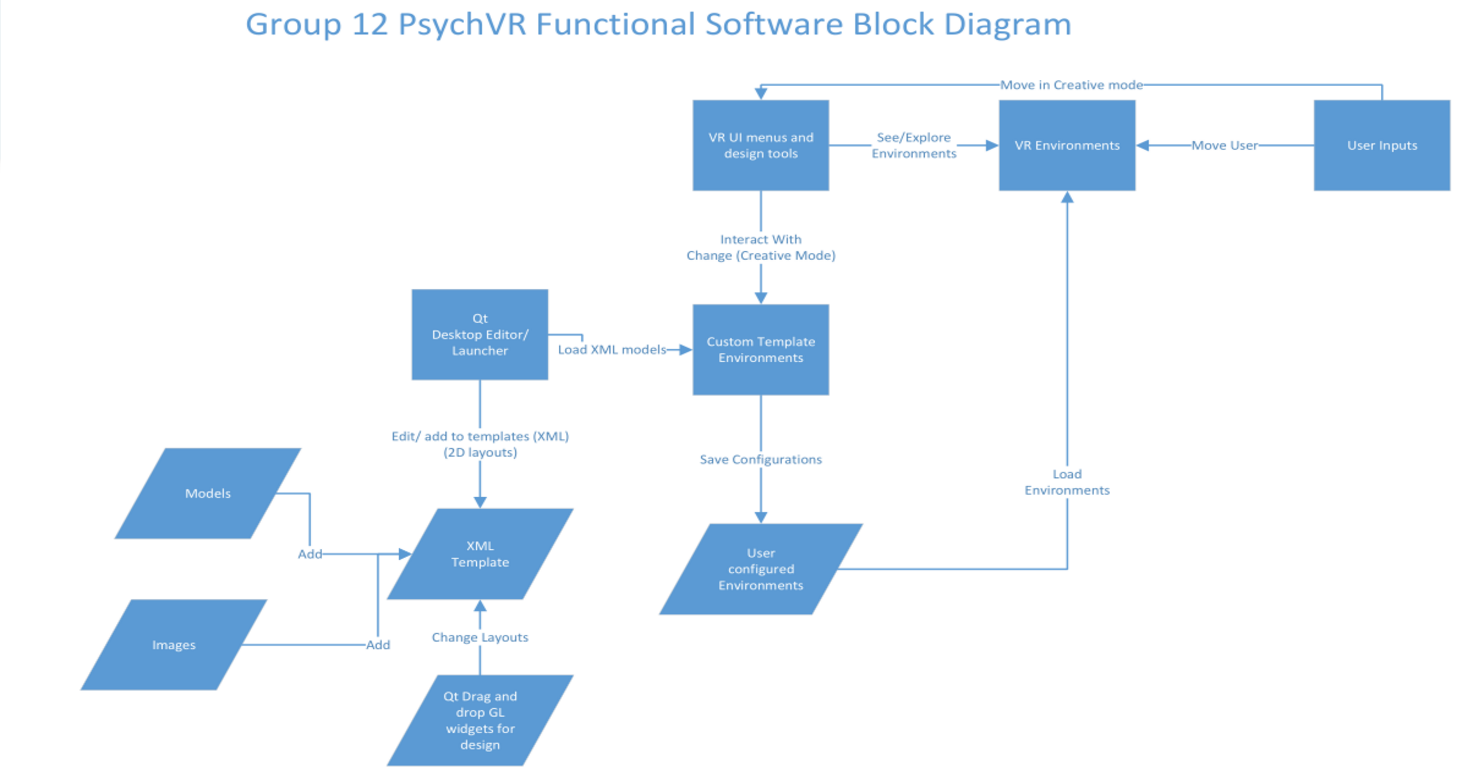
\includegraphics[width=\linewidth,height=\paperheight,keepaspectratio]{HardwareConfig.png}
	\caption{Hardware Block Diagram}
	%to ref fig number
	%Figure \ref{fig:block1} shows our blockDiagram.
	\label{fig:hblock}
	\end{figure}
	This diagram represents a hardware configuration of a typical VR system that our application would expect. This may change depending on the device we use, but is a good overview.
	\pagebreak
	\begin{figure}[H]
	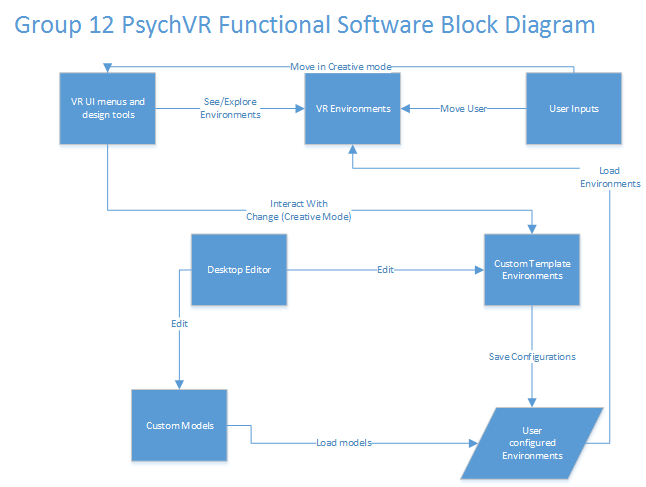
\includegraphics[width=\linewidth,height=\paperheight,keepaspectratio]{SoftwareConfig.png}
	\caption{Software Block Diagram}
	%to ref fig number
	%Figure \ref{fig:block1} shows our blockDiagram.
	\label{fig:sblock}
	\end{figure}
	This diagram represents the software design of our project and the various functional modules that should exist in order to fulfill the user interaction requirements. 
	The application will have two main modes of operation, edit mode and view mode. 
	\subsection{Qt Design Plan}
		\subsubsection{High Level Diagram}
		\subsubsection{Activity Diagram}
	\subsection{Unity Hierarchy}
		\subsubsection{High Level Design}
		\subsubsection{Activity Diagram}
		\subsubsection{Scene Shared Assets}
		
\pagebreak

%4. Administrative content
%G. Personnel and bibliography of related work, if any (mostly text)
%H. Facilities and Equipment (text, numbers, tables, charts, figures, diagrams)
%I. Consultants, subcontractors, and suppliers (mostly text)
%A. Budget and financing (text, numbers, tables, charts, figures, diagrams).
%B. Milestone chart for all activities related to the project
\section{Administrative Content}
\section{Budget and Financing}
	                    Financing is still being researched at this point.  Due to us not having a sponsor, we will either have to self-finance or contact people willing to help with funding.  Therefore, our budget and financing are extremely subject to change. We already have the hardware necessary to run virtual reality hardware, so that saves us the cost of building one ourselves (upwards of 1000 dollars). VR headsets vary in price, although our current target the Oculus Rift, costs 600 dollars. Using Unity Pro costs 75 dollars a month, so over the next 8 months it would add up to another 600 dollars. This totals to 1200 dollars for development and hardware. However, a number of on campus facilities also have virtual 
	                    reality headsets for testing and design purposes, including Sony’s VR headset Morpheus and a few Oculus Rifts.  If we can gain access to these facilities, we can cut down on hardware costs tremendously.  Additionally, if we can gain a sponsor or funding from UCF, we could potentially up our budget and invest in some newer VR 
	                    technology, and possibly be able to test for multiple platforms. The upper limit would be the Microsoft Hololens, which costs between 1500 dollars and 3000 dollars for a dev kit, while it is something we would 
	                    not be able to afford for this project alone, it could be something UCF would be interested in investing in.  
	                    
	                    \subsection{Summary:}
	                    Current Budget: Roughly \$1500.  \$600 for Dev Kit,
	                    \$600 for development Engine, \$200 for equipment and other software (in engine models, non-vr hardware such as controllers and cameras),\$100 for other
	                    expenses that could come up.
	                    
	                    \subsection{Funding}
	                    This is entirely self funded at the moment.  All of us have well-paying jobs in the 
	                    Orlando area, and would be able to spend \$500 if necessary.  However, hopefully we will be able to at the very least cut out the 
	                    \$600 Oculus Rift Dev Kit cost by using UCF facilities, and possibly cutting away the \$600 engine cost as well by settling on the limited free version of Unity.  
	%software licensing costs, cloud based service costs, code repo's, graphic design costs
	\section{Schedule}
	\begin{figure}[H]
	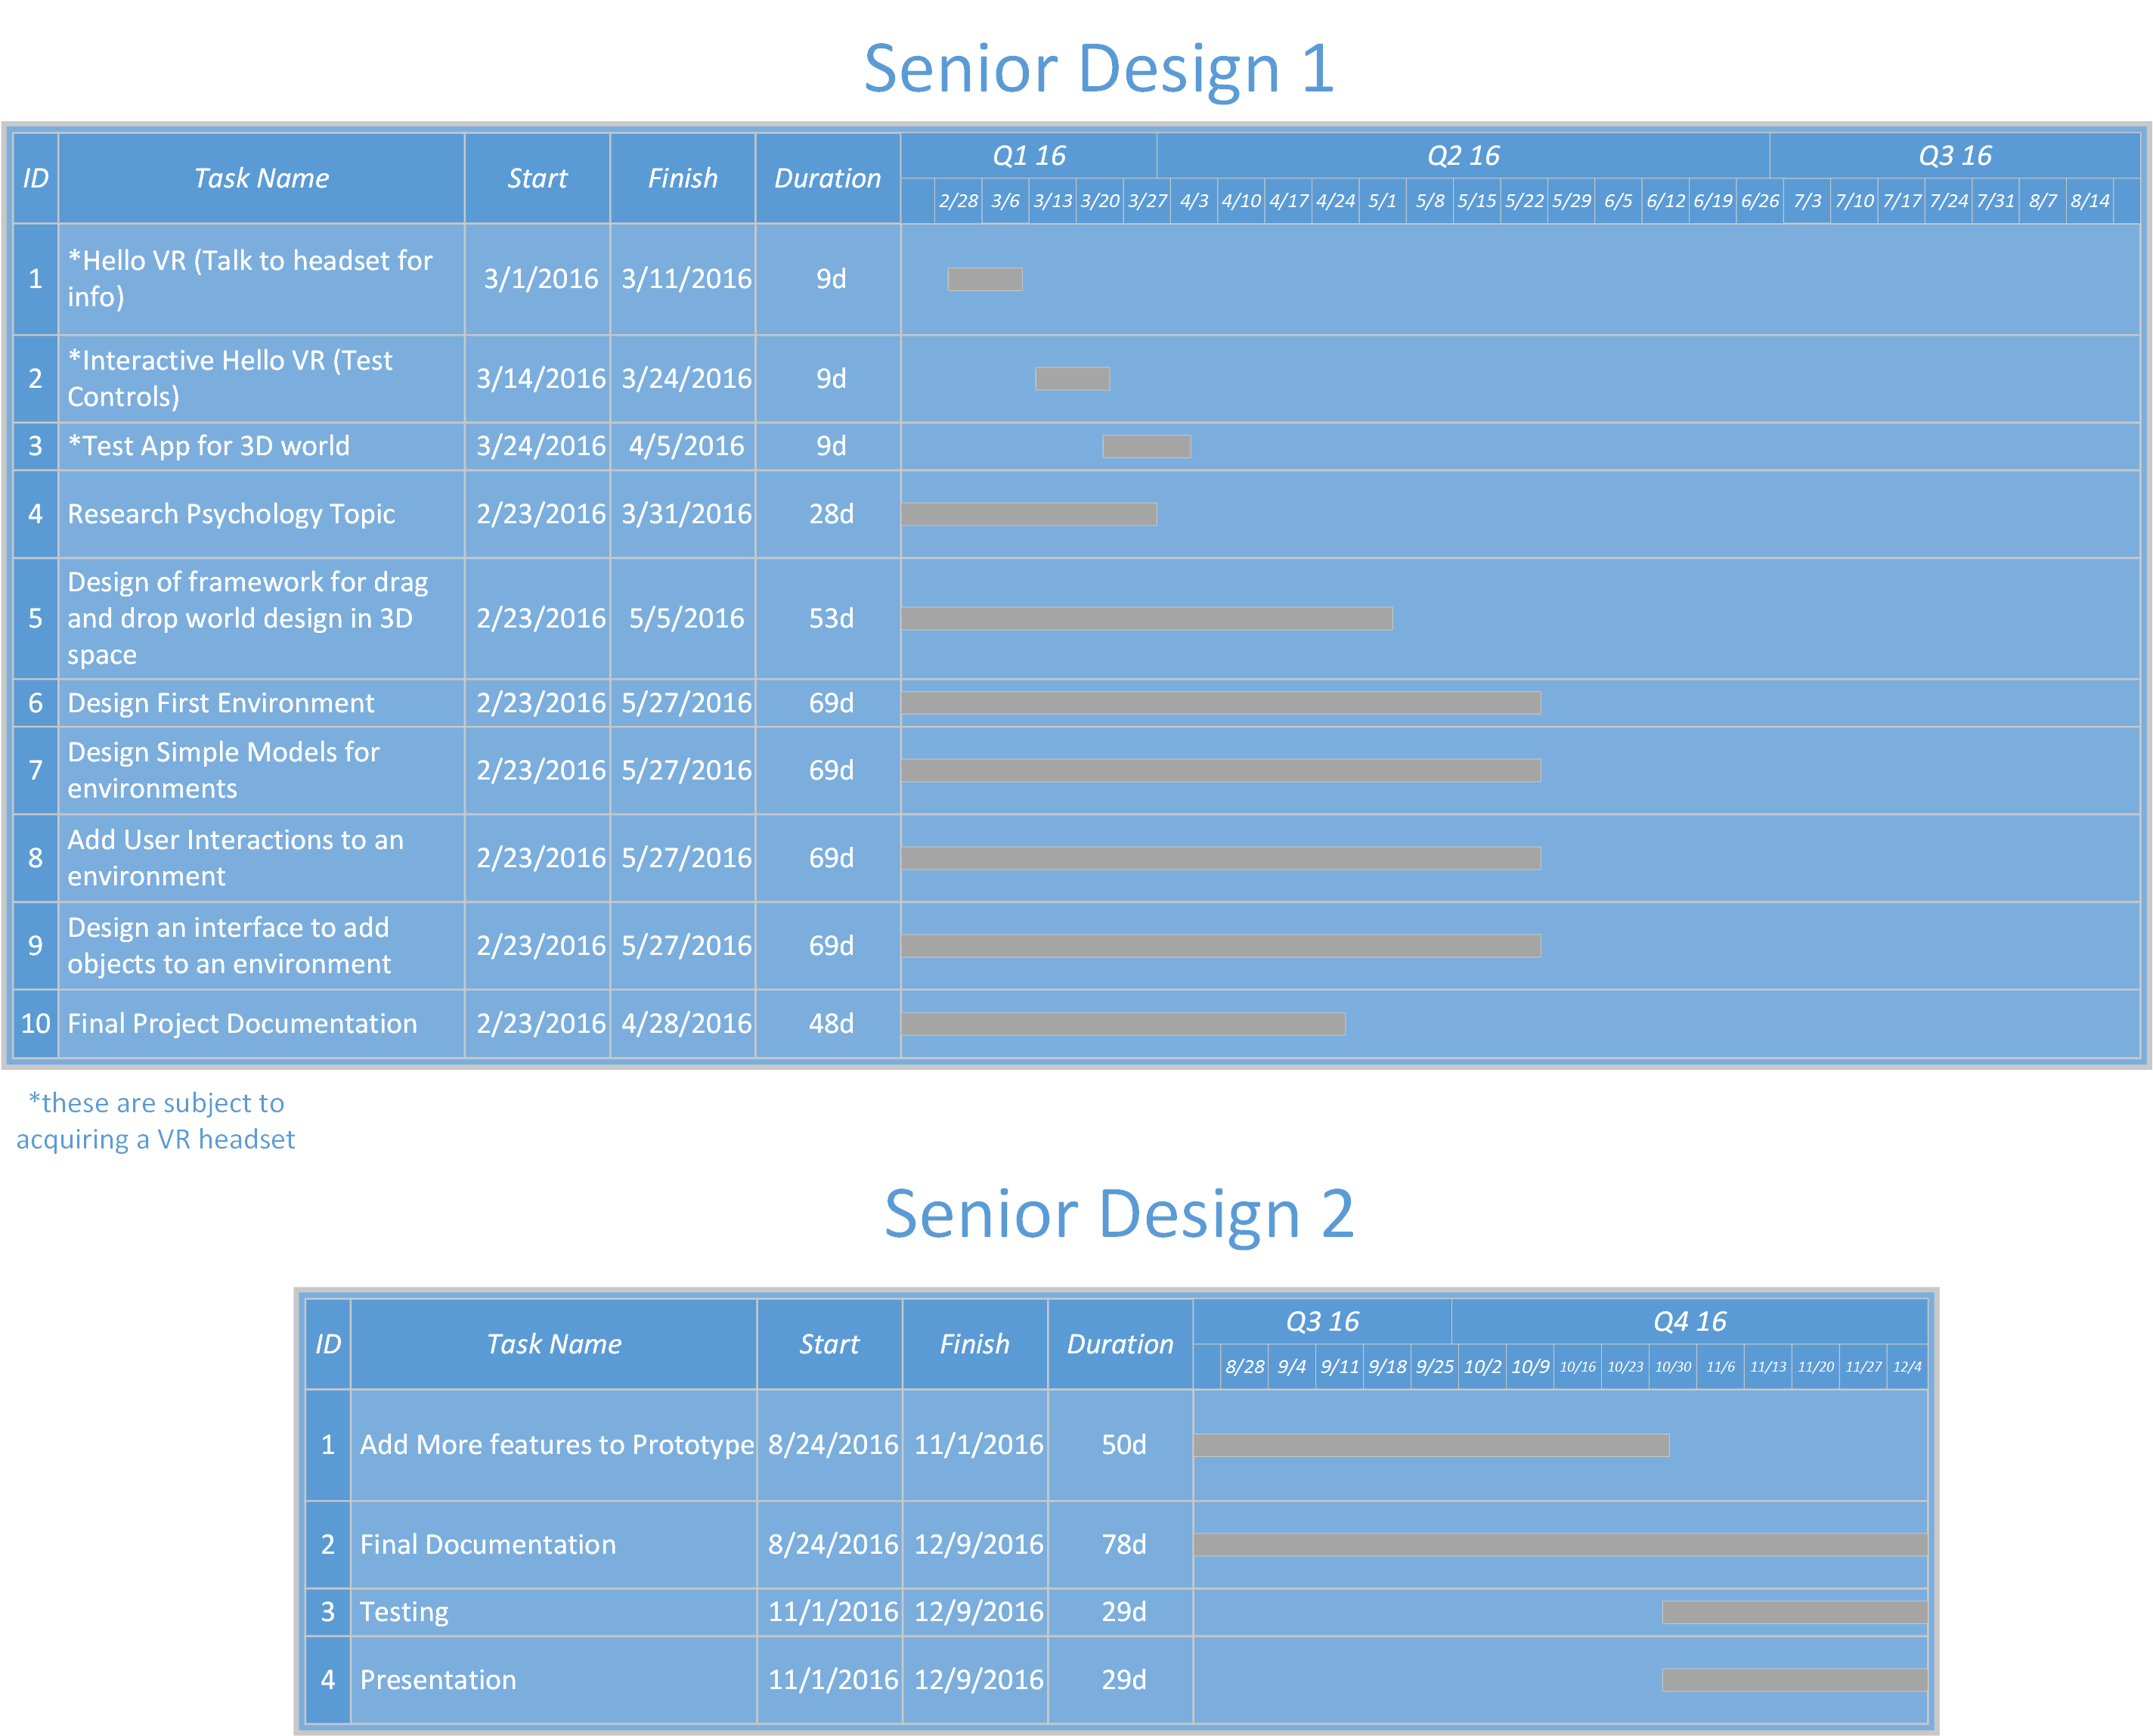
\includegraphics[width=\linewidth]{scheduleSR.png}
	\caption{Prototype Phase Gantt Chart:}
	%to ref fig number
	%Figure \ref{fig:block1} shows our blockDiagram.
	\label{fig:pchart}
	\end{figure}
	\section{Milestones}
	\subsection{Tech Milestones}
		\begin{itemize}
			\item Finding funding or available UCF facilities
			\item Obtaining Oculus Rift
			\item Obtaining Gear VR
			\item Obtaining LeapMotion
			\item Getting virtual reality hardware to display world
			\item Connecting user input to world
		\end{itemize}
	\subsection{Research Milestones}
		\begin{itemize}
			\item Choose the most important scenes to develop
			\item Testing with psychologists to confirm project is beneficial
		\end{itemize}
	\subsection{Development Milestones}
		\begin{itemize}
			\item Allowing for users to add models to world, and design said world
			\item Combining all aspects of project into cohesive whole
			\item Finalize and begin testing of project
		\end{itemize}
	\subsection{Overall Milestones}
		\begin{itemize}
			\item 
		\end{itemize}

\pagebreak
%5. Project Summary and conclusions.
\section{Project Summary and Conclusions}

\pagebreak
\pagenumbering{Alph}
\setcounter{page}{1}
%6. References
\section{References}

\bibliographystyle{mla}
\begin{thebibliography}{9}
\bibitem{stroke1}
Rettner, Rachael. "Stroke Therapy Gets Boost from Virtual Reality." LiveScience. TechMedia Network, 07 Apr. 2011. Web. 06 Apr. 2016.
\bibitem{dsmCaution}
"Cautionary Statement for DSM IV - TR." Cautionary Statement for DSM IV. N.p., n.d. Web. 10 Apr. 2016.
\bibitem {dsmPhobia}
"Diagnostic Criteria for 300.29 Specific Phobia." Diagnostic Criteria for 300.29 Specific Phobia. N.p., n.d. Web. 10 Apr. 2016.
\end{thebibliography}

%7. Appendices
\section{Appendices}

%A. Copyright permissions
\section{Copyright Permissions}

%B. Data-sheets (if necessary)
%C. Software (if necessary)
%D. Other
\section{Extras}

\end{document}
